\section{Design Details}
\label{sec:design}

\begin{figure*}
    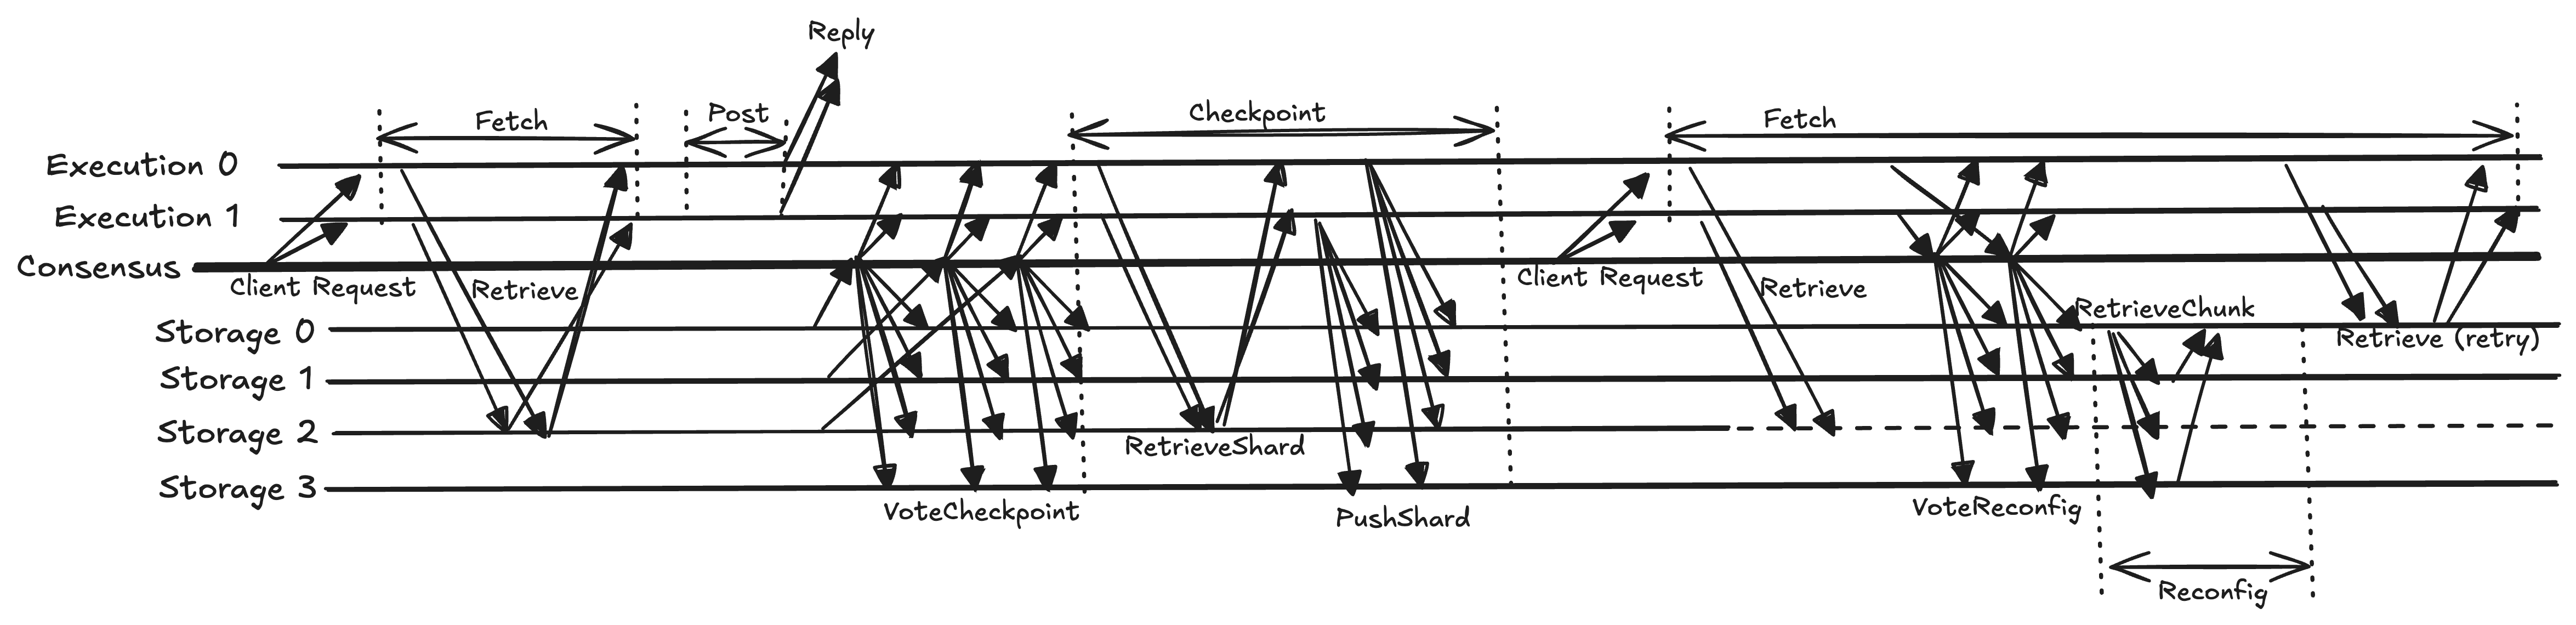
\includegraphics[width=\linewidth]{figures/message-flow}
    \caption{Message flow.}
    \label{fig:message-flow}
\end{figure*}

\begin{figure}
    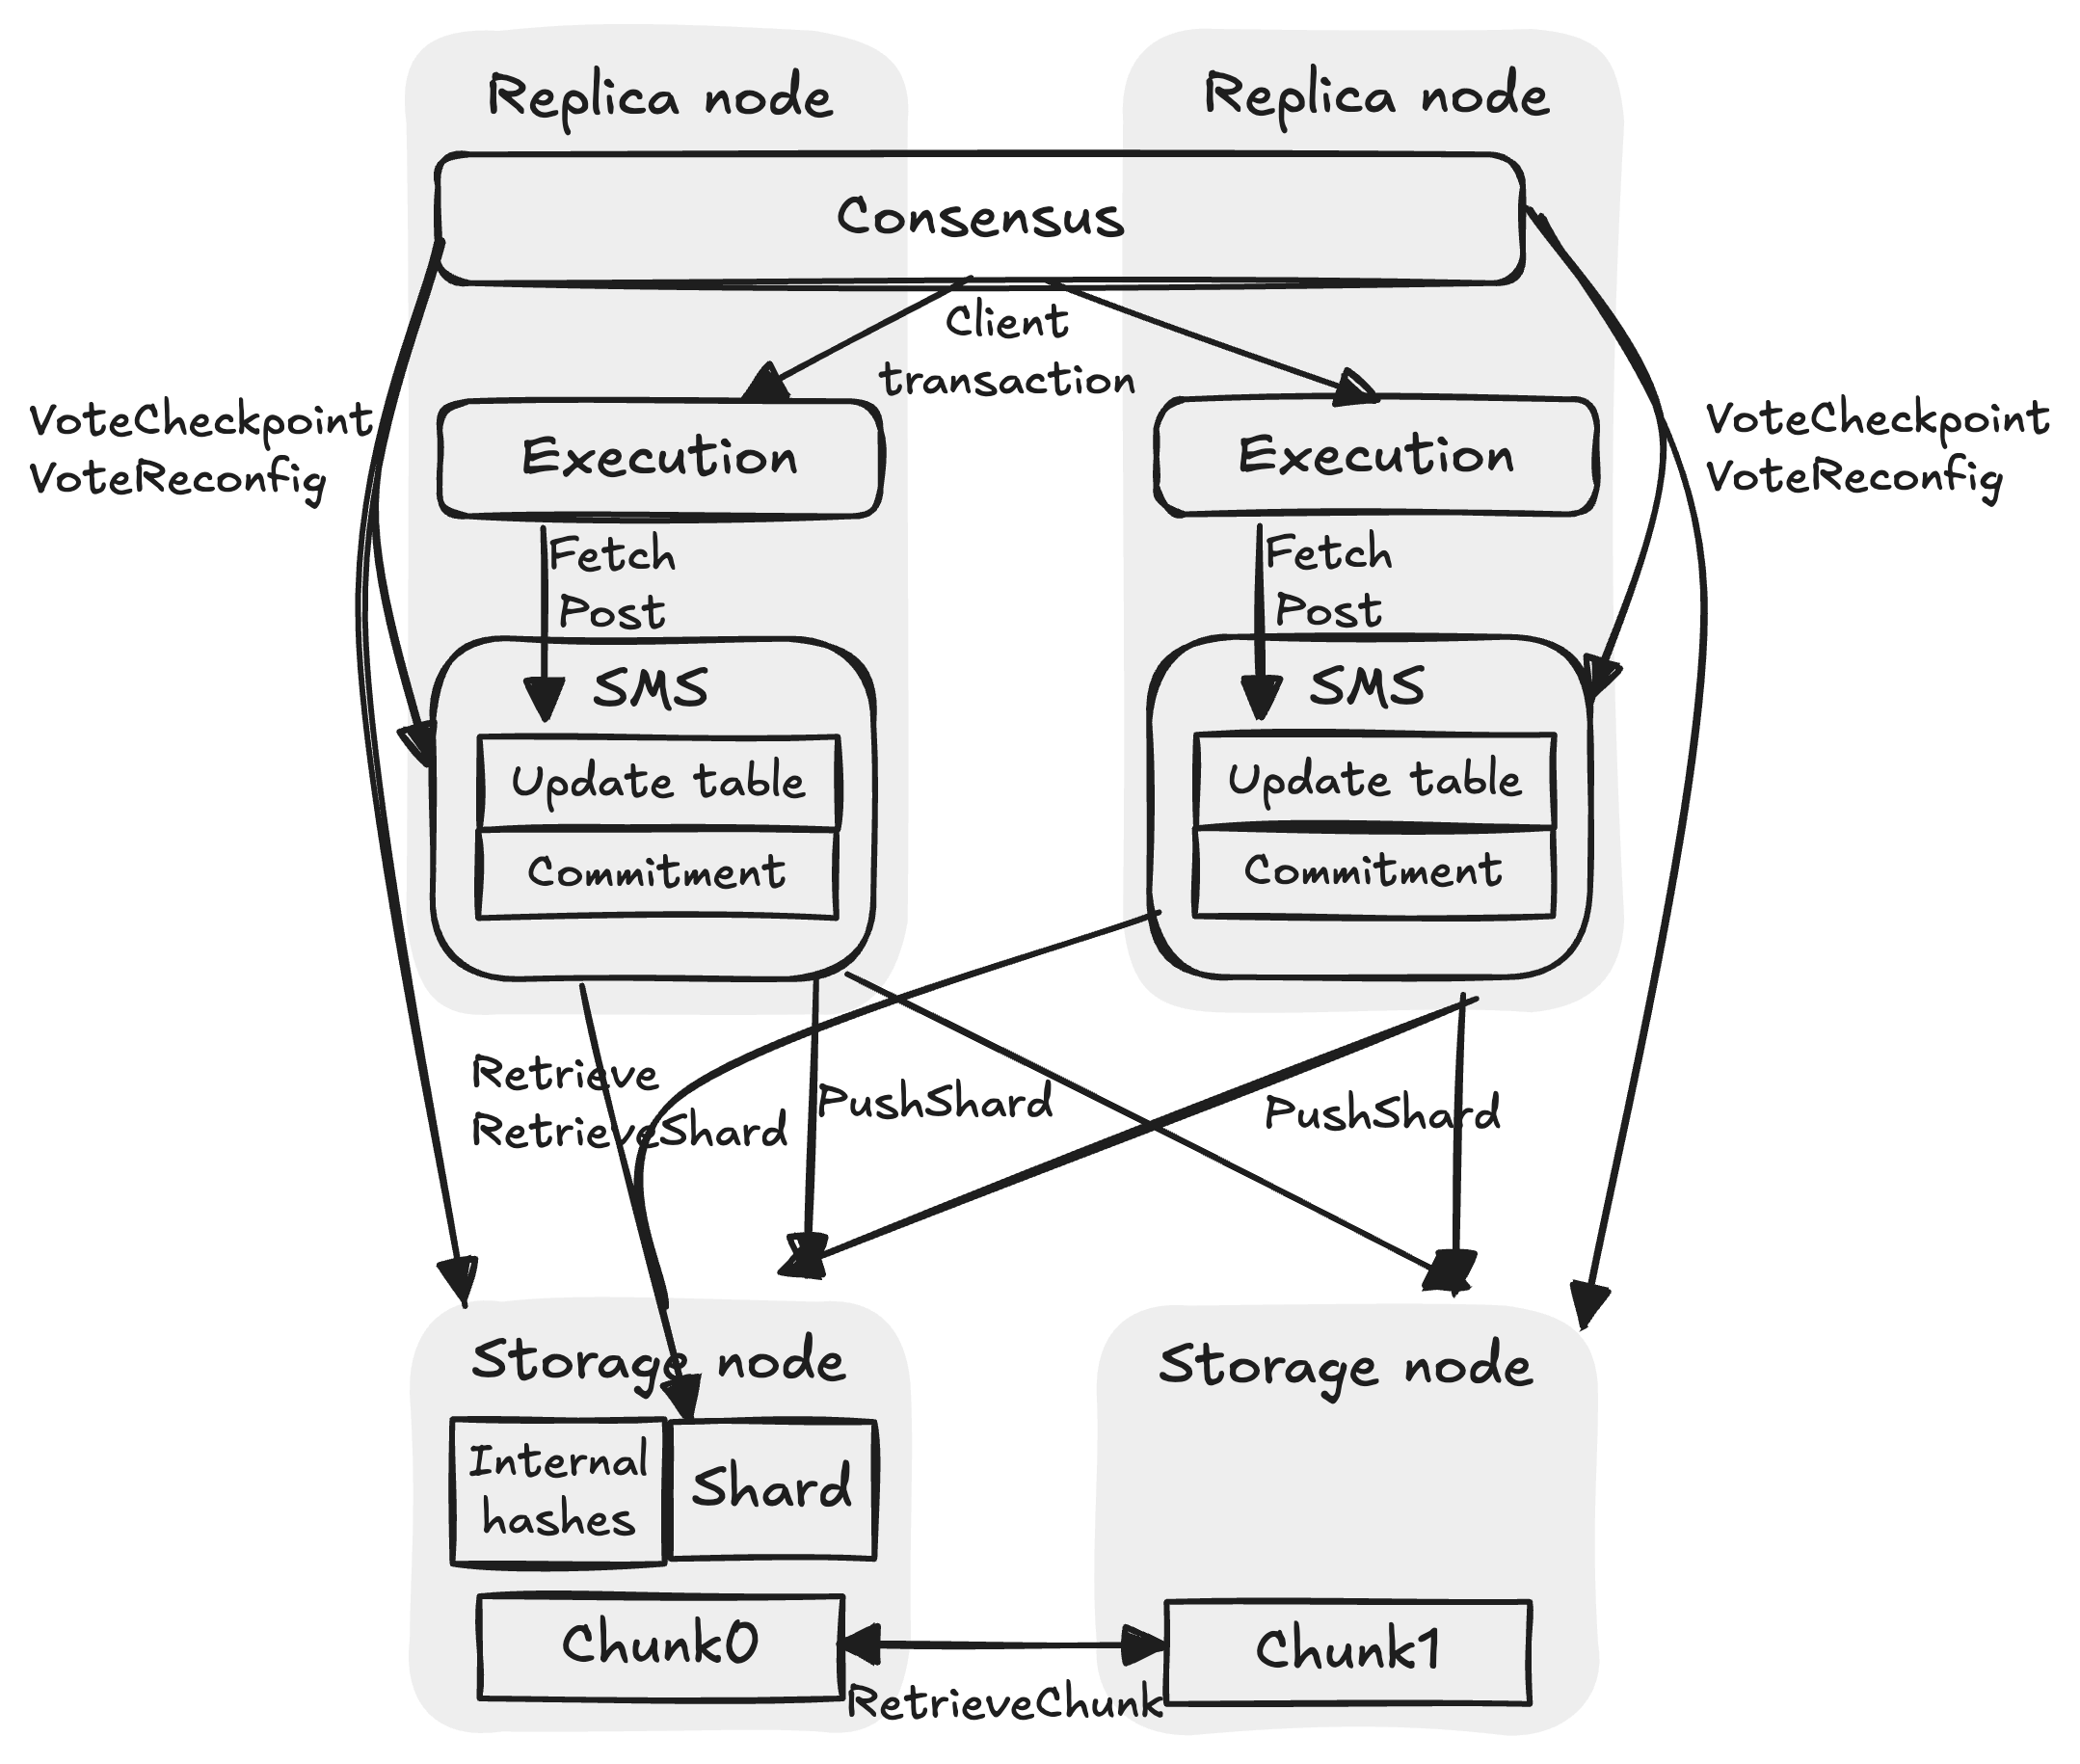
\includegraphics[width=\linewidth]{figures/node-states}
    \caption{Node states.}
    \label{fig:node-states}
\end{figure}

\begin{table*}
\centering
\small
\renewcommand{\arraystretch}{1.2}
\begin{tabular}{@{}lll@{}}
\toprule
\textbf{Channel} & \textbf{Message} & \textbf{Data} \\
\midrule
\multirow{7}{*}{Storage nodes RPC}
    & \retrieve{} request   & round, key \\
    & \retrieve{} response  & round, key, value, inclusion proof \\
    & \retrieves{} request  & round, shard ID \\
    & \retrieves{} response & round, shard ID, shard data \\
    & \getsc{} request      & round, shard ID \\
    & \getsc{} response     & round, shard ID, storage node ID, chunk data \\
    & \pushss{}             & round, shard ID, shard data \\
\addlinespace
\multirow{2}{*}{Atomic broadcast}
    & \votec{}              & round, storage node ID, shard commitments from previous round \\
    & \voter{}              & epoch, round, replica node ID, nonce \\
\bottomrule
\end{tabular}
\caption{SMS messages grouped by channel.}
\label{tab:messages}
\end{table*}

In this section, we detail the data structures and the algorithms of the replica and the storage nodes and the protocol between them.
The messages used in the protocol are summarized in \autoref{tab:messages}.
The messages are categorized into two channels according to how they are delivered.
The storage nodes RPC channel is unordered and unreliable point-to-point communication, and the storage nodes respond to the requests to serve and update their stored data.
The \retrieve and \retrieves requests and \pushss are sent by the replica nodes, while the \getsc requests are sent by the peer storage nodes.

The atomic broadcast channel is a reliable total order broadcast provided by the underlying BFT atomic broadcast protocol.
The broadcast messages are sent by the replica nodes submitting them as client transactions to the atomic broadcast protocol.
Both types of messages are subscribed by both the replica and storage nodes.
The storage nodes can subscribe to the messages via relaying by their trusted replica nodes, i.e., the replica nodes hosted by their operators.

Every message contains a \emph{round} number, which indicates the checkpoint round the message belongs to.
The round number starts from 0 at system startup and increments by one after each checkpoint round.
The \voter messages also contain an \emph{epoch} number to indicate the number of reconfigurations that have happened, because reconfiguring to the same round may happen multiple times.

\subsection{Randomized Replication Scheme}

The SMS first maps each key to a shard ID using a hash function.
Next, for each shard, it needs to set up full copies on the responsible storage nodes for retrieval.
We call the mapping from shards to their responsible nodes the \emph{placement}.
Suppose there are $N$ storage nodes and $k$ shards, we want the placement to:
\begin{itemize}
    \item Replicate each shard to exact $r$ storage nodes;
    \item Balance the load across all storage nodes, that is, each storage node should be responsible for at most $\lceil rk/N \rceil$ shards, and
    \item The probability that each node is responsible for a given shard is uniform across all nodes.
\end{itemize}
To achieve these goals, we choose a simple Markov-chain algorithm~\cite{kannan1999simple} to generate the placement.
The algorithm starts with an initial placement that assigns each shard $i$ to $r$ (circular) consecutive storage nodes starting with node $i \mod N$.
Then, it repeatedly selects two shards and two storage nodes at random so that each of the nodes is responsible for exactly one of the shards, and swaps the two shards between the two nodes.
After sufficient number of swapping, the placement converges to a uniform distribution.
It also satisfies the replication and load balancing requirements, because the initial placement satisfies them and each swap preserves them.

The randomization procedure is performed with a seeded pseudo-random number generator whose seed is fed from the nonces of $f+1$ \voter messages.
Each node can independently compute the placement for the shards with the seed during each reconfiguration.
These \voter messages are agreed upon via atomic broadcast, so the placement is consistent across all nodes.
Because at least one of the $f+1$ replica nodes sending the \voter messages is correct, the seed is unpredictable to the adversary.

\subsection{Storage Nodes}

The storage nodes are designed as ``dumb'' storage servers with minimal logic.
The stored unit is a shard, and the storage nodes store a shard of a round when it receives $f+1$ matching \pushss messages from distinct replica nodes, ensuring the integrity of the shard.
Then, the stored shard can be retrieved in three different ways: via \retrieve, \retrieves, and \getsc requests, and the storage nodes store the shard in two formats to serve these requests.
Every storage node encode each stored shard into $3f+1$ chunks with the RS code, and store the chunk corresponding to itself, and they serves the \getsc requests with these chunks.
The $r$ responsible storage nodes for a shard also store a full copy of the shard and the Merkle tree constructed for the shard.
They serve the \retrieves requests with the full shard, and for the \retrieve requests, they first prove the inclusion of key value pair with the Merkle tree and then return the value with the inclusion proof.


While not strictly necessary, the storage nodes can also subscribe to the checkpoint signals, and only accept \pushss messages for the current checkpoint round.

\subsection{Replica Nodes}

The execution layer sequentially processes the ordered messages delivered by the atomic broadcast protocol.
If the message is a client transaction, it executes the transaction and accesses the state by calling \fetch and \bump according to the application logic.
Otherwise, if the message is an SMS message, it forwards the message to the SMS for processing.
The SMS maintains the current checkpoint round, an update table and a cache on the replica nodes.
On \bump operations, the SMS records the updated keys and their new values in the update table.
On \fetch operations, the SMS first checks the update table for the requested key and return the value directly if found.
If not found, it checks the cache and lastly resorts to sending \retrieve requests to the storage nodes on cache miss.
The \retrieve requests are batched to reduce communication overhead.
After getting the responses, the SMS verifies the values and proofs against the shard commitment, updates the cache, and returns the values to the execution layer.

The SMS suspects liveness failure if the \retrieve requests are not (correctly) responded within a timeout.
In this case, it increments the epoch and sends \voter messages with its current checkpoint round and a random nonce to the atomic broadcast protocol.

The SMS also records the forwarded \votec and \voter messages.
When it collects $2f+1$ \votec from distinct storage nodes for round $c'$ greater than its current checkpoint round $c$, it enters checkpoint round $c'$.
If $c'>c+1$, it returns \forward to the execution layer to skip to the version at round $c'-1$.
It snapshots the update table before handling further \bump operations.
It is crucial that the \votec messages are ordered respect to the client transactions to ensure consistent checkpointing across all replica nodes.
Then, it sends \retrieves requests to the storage nodes to retrieve the shards at round $c'-1$ and verify them against the shard commitments in \votec messages.
The \votec messages are designed to include the shard commitments to ensure that nodes can verify the retrieved shards independently, even if they are absent from the previous checkpoint round.
And then, SMS applies the relevant updates in the update table snapshot to the retrieved shards.
SMS then computes the new shard commitments and send \pushss messages with the new shards to the storage nodes.
The update table snapshot is kept until the SMS pushes all the shards for round $c'$.

When SMS collects $f+1$ \voter messages with matching epoch and round from distinct replica nodes, it reseeds the randomized placement scheme with the nonces and redirects the subsequent \retrieve requests to the new responsible storage nodes.
